% !TEX root = ../my-thesis.tex
%
\chapter{Architettura della soluzione}
\label{sec:methods}


Il lavoro di questa tesi si basa sull'intuizione che i risultati raggiunti nell'ambito della KBP mediante \textit{Distant Supervision} (Sez. \ref{sec:literature_review:information_extraction:distant_supervision}), gli sviluppi introdotti dalla nuova tecnica di \textit{Data Programming} (Sez. \ref{sec:literature_review:data_programming}) e l'efficienza dimostrata dalle \textit{Bidirectional Long Short Term Memory Network} (\textit{Bi-LSTM}) (Sez. \ref{sec:methods:training}) con input sequenziali come il testo libero, possano essere combinati per ottenere risultati allo stato dell'arte nel popolamento di basi di conoscenza Linked Data. 
In particolare il fine è quello di dare una dimostrazione empirica di come una base di conoscenza Linked Data come DBpedia possa essere popolata con nuove triple, composte da predicati già definiti in un'ontologia OWL (DBpedia Ontology), analizzando testi enciclopedici scritti in linguaggio naturale (Wikipedia) e sfruttando l'insieme di triple già esistenti (distant supervision) ed euristiche specifiche (weak supervision) per costruire un insieme di frasi automaticamente etichettate utilizzato per allenare un classificatore di tipo Bi-LSTM.

La tecnica di data programming viene implementata nel progetto Snorkel di cui si fa uso in questo progetto. Grazie a Snorkel è possibile gestire l'intero processo di classificazione a partire dal parsing del corpus fino all'allenamento supervisionato di un classificatore. Il processo viene trattato come un problema di classificazione binaria in cui per un segmento di testo si deve valutare se è adatto o meno a rappresentare una relazione Linked Data. Le triple vengono estratte dalle sole proposizioni testuali classificate positivamente.

Vista la totale indisponibilità di basi di verità etichettate naturalmente, Snorkel ne consente la produzione automatica con varie tecniche di weak supervision implementate dalle \textit{labeling functions}. La distant supervision, la labeling function su cui si ripone maggiore affidamento in questo lavoro, viene potenziata dall'utilizzo di altre funzioni di labeling specifiche.
Con la definizione di semplici labeling functions basate su parole chiave si prevede di aumentare la copertura della distant supervision e limitarne gli errori. In tal caso si raggiungerebbe un risultato pratico importante: l'estrazione di triple potrebbe essere favorita dall'uso di liste di parole chiave la cui produzione può essere fatta manualmente "a basso costo" o automaticamente, instaurando un processo di estrazione iterativamente perfezionabile nel tempo.

Il corpus testuale utilizzato è in lingua Inglese, ma è potenzialmente estendibile a qualsiasi linguaggio naturale supportato dal parser NLP che si decide di utilizzare.

Nel progetto viene impiegata come fonte dati per la distant supervision la stessa base di conoscenza che si vuole popolare: DBpedia. Il punto di accesso per effettuarne l'interrogazione è lo SPARQL Endpoint. Il linguaggio SPARQL viene impiegato sia per il reperimento dei dati campione, che per inferire metadati di interesse sui predicati presi in esame. 

Le etichette prodotte dalle varie labeling function vengono analizzate statisticamente da un algoritmo generativo che ne restituisce le probabilità marginali che vengono a loro volta sfruttate per l'allenamento di un classificatore discriminativo.

Il classificatore ottenuto può essere utilizzato per processare nuovo testo e riconoscere le menzioni testuali dalle quali estrarre delle nuove triple.

Il task di LDKBP si compone di un insieme potenzialmente molto vasto di predicati OWL. Per tale ragione si è progettato un sistema con una struttura \textit{pipeline} adatto ad essere facilmente configurato e ripetutamente eseguito.

\begin{figure}[htb]
	\fbox{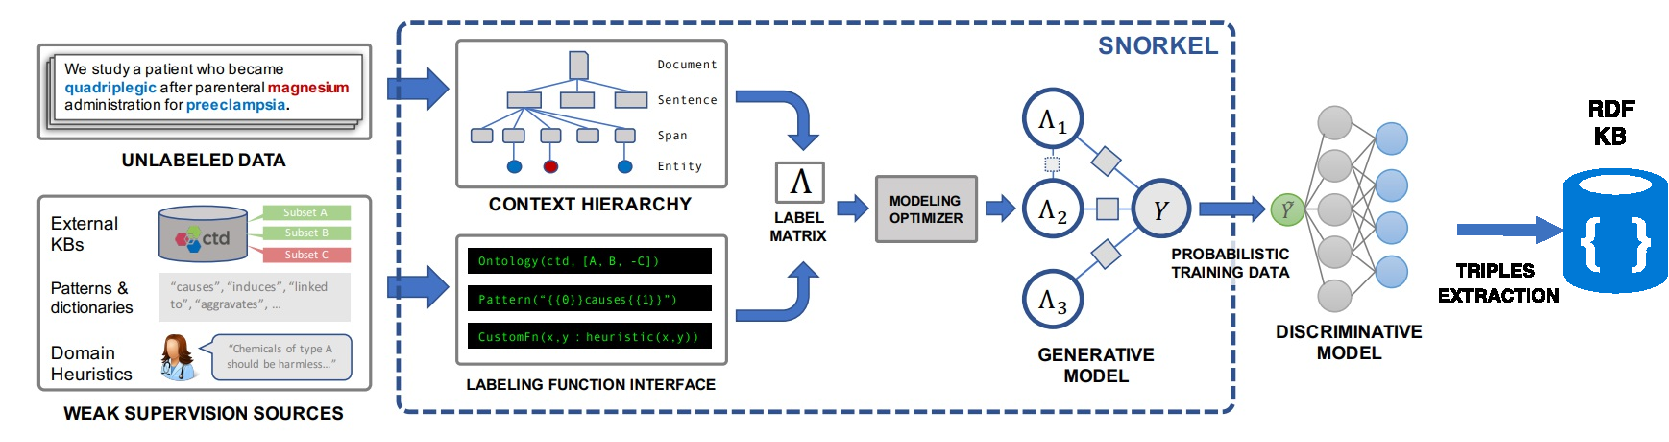
\includegraphics[width=\textwidth]{gfx/sentimantic_diagram.pdf} }
	\caption{Diagramma del progetto.}
	\label{fig:methods:project_diagram}
\end{figure}

Nel corso di questo capitolo si descrive l'ambiente, la configurazione e il processo di funzionamento della pipeline (Fig. \ref{fig:methods:project_diagram}) che si compone dei seguenti passi fondamentali:

\begin{itemize}

\item parsing NLP del corpus Wikipedia: per ogni frase rilevata si memorizzano features testuali (Sez. \ref{sec:methods:text_extraction} e \ref{sec:methods:parsing_nlp});

\item inferenza dei tipi di Named Entity che caratterizzano \textit{dominio} e \textit{range} di ogni predicato in input (Sez. \ref{sec:methods:candidate_inference});

\item etichettamento delle frasi candidate con labeling function  (Sez. \ref{sec:methods:labelling});

\item ottimizzazione dell'insieme etichettato e training del modello di classificazione (Sez. \ref{sec:methods:training});

\item estrazione delle triple dal testo classificato positivamente (Sez. \ref{sec:methods:triples_extraction}).
\end{itemize} 















\section{Configurazione e Ambiente}
\label{sec:methods:config}
Il progetto è strutturato sotto forma di pipeline che ha come input un file di configurazione che descrive:
\begin{itemize}
\item l'URI del corpus testuale;
\item l'URL dello SPARQL Endpoint della base di conoscenza da interrogare;
\item una lista di predicati Linked Data per cui estrarre le triple e per ciascuno (opzionalmente):
\begin{itemize}
\item una lista di parole chiave positive,
\item una lista di parole chiave negative,
\item una lista di indici di documenti del corpus da usare come test (e che quindi non vengono inclusi nell'insieme di training).
\end{itemize}
\end{itemize}

Il software maggiormente utilizzato nella pipeline è, come già detto, Snorkel. Esso è scritto in linguaggio \textit{Python} e integra a sua volta librerie e servizi di terze parti per: la gestione del database, il parsing NLP, il machine learning e la produzione di "gold label" per la valutazione.
Nel caso specifico si è scelto di utilizzare il DBMS \citetitle{postgresql} \cite{postgresql}, l'ORM \citetitle{sql_alchemy} \cite{sql_alchemy}, il parser \citetitle{spacy} \cite{spacy}, la libreria di machine learning \citetitle{tensorflow} \cite{tensorflow} e il tool di annotazione \citetitle{brat} \cite{brat}.

Altre librerie e servizi di terze parti utilizzati e non integrati in Snorkel sono: il progetto \textit{WikiExtractor} \cite{WikiExtractor} per la pulizia del dump testuale, la libreria \textit{RDFLib} \cite{RDFLib} per l'interrogazione SPARQL, la libreria \textit{Wikipedia} \cite{wikipedia_API} per il download del corpus, la libreria \textit{TextaCy} \cite{textacy} per funzionalità di NLP aggiuntive e \textit{DBpedia Lookup} \cite{dbpedia_lookup} per l'entity linking.


Per facilitare lo sviluppo, il deploy e il test del sistema prodotto si è deciso di modellare un'infrastruttura di \textit{container Docker} \cite{docker} che permette di:
\begin{itemize}
\item replicare le computazioni in ambienti virtuali sempre uniformi;
\item mantenere le performance di un ambiente non virtualizzato \cite{Felter2015AnUP};
\item fare deploy dell'infrastruttura con pochi comandi su qualsiasi macchina che abbia installato Docker e sia connessa al \textit{Docker Cloud};
\item scalare e bilanciare i servizi in maniera semplice;
\item monitorare e riavviare automaticamente servizi in stato di errore.
\end{itemize}

I servizi che compongono l'infrastruttura sono: 
\begin{itemize}
\item l'ambiente Python con le necessarie dipendenze software;
\item il database PostgreSQL;
\item DBpedia Lookup;
\item il tool di annotazione \textit{Brat}.
\end{itemize}
Grazie al componente \textit{Stack} di Docker è possibile configurare l'intero sistema in un singolo file \textit{YAML} (Snippet \ref{lst:results:docker1}).

\lstset{ basicstyle=\LSTfont, columns=fullflexible, xleftmargin=5mm, framexleftmargin=5mm, numbers=left, stepnumber=1, breaklines=true, breakatwhitespace=false, numberstyle=\footnotesize, numbersep=5pt, tabsize=2, frame=lines, captionpos=b}
\begin{lstlisting}[frame=single, caption={File docker-compose.yml di configurazione dell'infrastruttura Docker},label={lst:results:docker1},]  
version: '3'
services:
  postgres:
    image: postgres
    environment:
      POSTGRES_PASSWORD: sentimantic
      POSTGRES_USER: sentimantic
      PGDATA: /var/lib/postgresql/data/sentimantic
    ports:
      - "54320:5432"
    deploy:
      replicas: 1
      restart_policy:
        condition: on-failure
    volumes:
      - ./.database:/var/lib/postgresql/data/sentimantic
  lookup:
    image: dbpedia/lookup
    command: java -jar /opt/lookup/dbpedia-lookup-3.1-jar-with-dependencies.jar /opt/lookup/2015-10/
    deploy:
      replicas: 32
      update_config:
        parallelism: 32
        delay: 20s
      restart_policy:
        condition: on-failure
    ports:
      - "1111:1111"
  py2Env:
    image: lorenzoranucci/sentimantic
    build: ./
    depends_on:
      - postgres
      - lookup
    tty: true
    volumes:
      - ./:/home/Sentimantic
  brat:
    image: cassj/brat
    volumes:
      - ./snorkel/snorkel/contrib/brat/brat-v1.3_Crunchy_Frog/data:/bratdata
      - ./snorkel/snorkel/contrib/brat/brat-v1.3_Crunchy_Frog/configurations:/bratcfg
    environment:
      BRAT_PASSWORD: brat
      BRAT_USERNAME: brat
      BRAT_EMAIL: lorenzofranco.ranucci@gmail.com
    ports:
      - "8001:80"

\end{lstlisting}   

Il container con le dipendenze Python e il progetto sviluppato è stato generato scrivendo un \textit{Dockerfile} che specializza l'immagine Docker rilasciata da \textit{Anaconda}: un progetto per la gestione delle dipendenze e virtualizzazione degli ambienti consigliato nella documentazione di Snorkel per la sua installazione.

Il database PostgreSQL è stato scelto seguendo la documentazione di Snorkel poiché consente, a differenza del database \textit{SQLite} impostato di default, una computazione parallela. 
 





















\section{Estrazione del corpus}
\label{sec:methods:text_extraction}
Il primo passo della pipeline è quello di predisporre l'input principale: il corpus testuale.

Wikipedia è una delle risorse enciclopediche del web più popolari, è gratuita ed è costantemente aggiornata nel tempo da una vasta comunità. Non solo può essere consultata liberamente via browser, ma il suo contenuto può essere scaricato con API o in blocco grazie ai dump periodici messi a disposizione pubblicamente. 

La forma linguistica uniforme e poco complessa del contenuto di Wikipedia si presta ottimamente al lavoro in oggetto, tuttavia il corpus è potenzialmente intercambiabile con quello di altre fonti.

Per il download del testo di training si è scelto di adottare i dump periodici, mentre per la selezione degli articoli su cui effettuare i test si sono sfruttate le API. I dump, a differenza dei dati delle API, contengono elementi di markup e link di disturbo per l'analisi NLP. Per questo motivo è stata necessaria una prima fase di pulizia portata a termine grazie al progetto WikiExtractor dell'\textit{Università di Pisa}. 

Il testo scaricato è stato infine memorizzato su file XML secondo una semplice struttura in cui i nodi di primo livello rappresentano i singoli documenti e contengono a loro volta i nodi \textit{id} e \textit{text}.

\begin{figure}[htb]
	\fbox{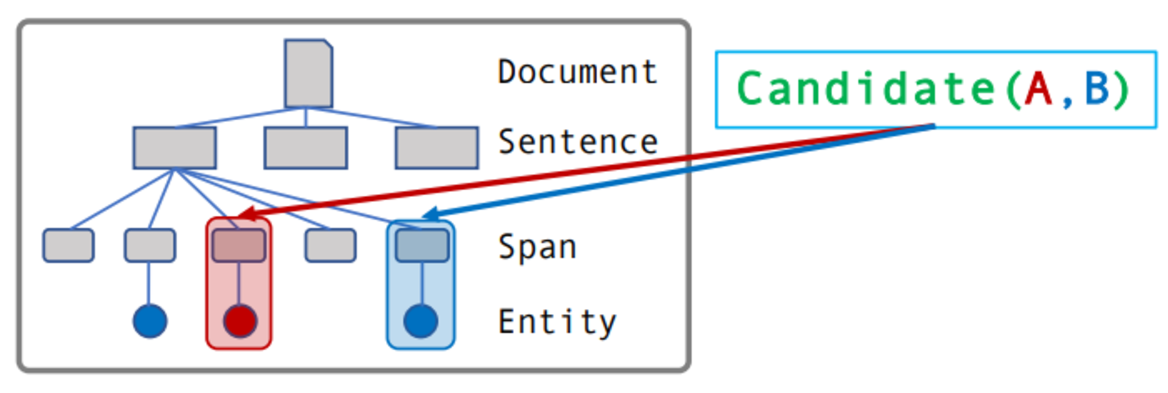
\includegraphics[width=\textwidth]{gfx/candidate.pdf}  }
	\caption{Modellazione del corpus in Snorkel.}
	\label{fig:methods:snorkel_struct}
\end{figure}

In Snorkel il corpus viene memorizzato come una gerarchia di oggetti della classe e tabella \textit{Context}. Attualmente la gerarchia predefinita per il testo è: \textit{Context -> Document -> Sentence -> Span} (Fig. \ref{fig:methods:snorkel_struct}).
Questa struttura viene definita e memorizzata nel database nelle successive operazioni della pipeline: nella fase di parsing si ottengono gli oggetti Document e Sentence e nella fase di candidate extraction si determinano le menzioni di entità Span che delimitano i segmenti di testo \textit{Candidate} per cui si vuole determinare un etichettamento.




\section{Parsing NLP}
\label{sec:methods:parsing_nlp}

Le triple Linked Data che si vogliono estrarre dal testo sono modellate secondo quella che in ambito linguistico viene chiamata \textit{proposizione}. Secondo la linguistica una proposizione può costituire una frase semplice se separata dal resto del discorso con simboli di \textit{interpunzione forte} o comporre insieme ad altre proposizioni una frase complessa. 

L'idea intuitiva è quella di analizzare tutte le frasi del corpus e distinguerne quelle che hanno features linguistiche tali da discriminare un particolare predicato e rappresentare un'asserzione Linked Data.

Per poter fare computazioni sul corpus risulta conveniente, come prima operazione, suddividere il corpus in frasi (semplici o complesse) che chiameremo d'ora in poi \textit{sentence}. Per ogni sentence si estraggono informazioni sintattiche, lessicali e semantiche che vengono poi sfruttate nei successivi passaggi della pipeline. 

\begin{figure}[htb]
	\fbox{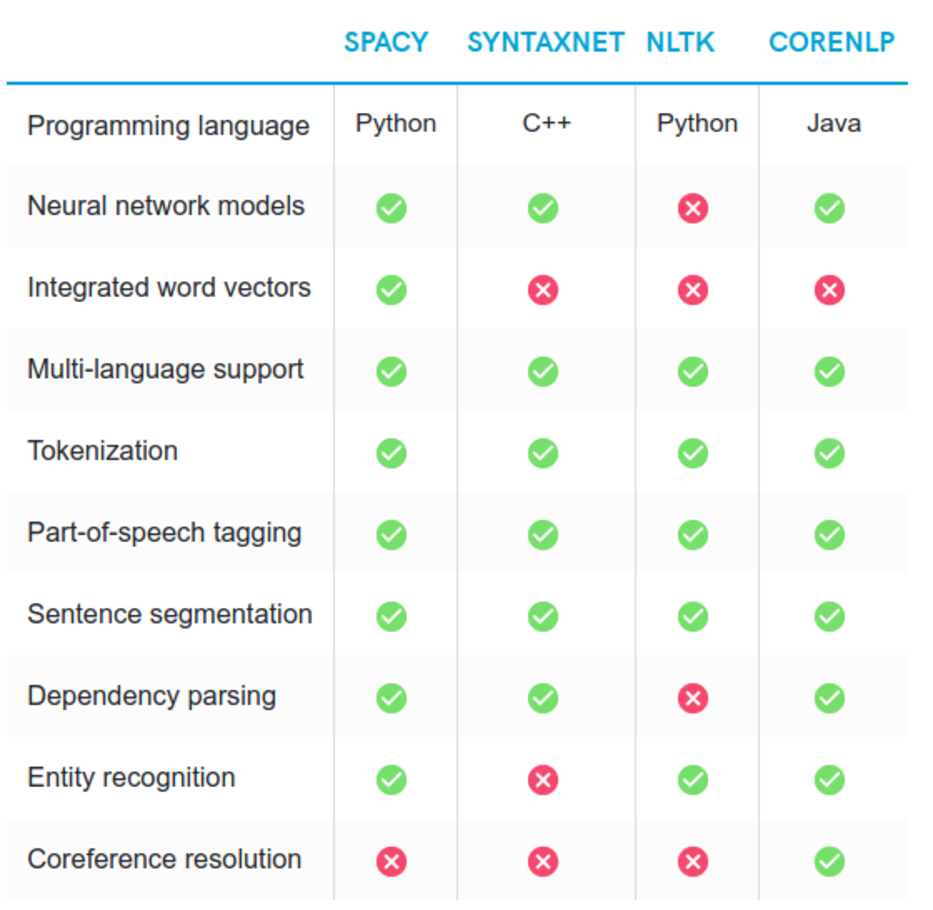
\includegraphics[width=\textwidth]{gfx/nlp_comparison.pdf} }
	\caption{Confronto delle funzionalità dei parser NLP più popolari.}
	\label{fig:methods:nlp_comparison}
\end{figure}

Il sistema Snorkel entra in azione sin da questo punto. Esso infatti integra due parser NLP: SpaCy e CoreNLP. Come dimostrato in \cite{Choi2015ItDD}, SpaCy è ad oggi il parser più veloce al mondo ed è quindi indicato il suo utilizzo con corpus molto grandi come in questo progetto. Non richiede comunque grandi compromessi in termini di precisione, rientrando infatti nell'1\% dei parser più precisi \cite{Spacyfacts}. Fornisce inoltre un output di feature linguistiche pensato per essere utilizzato come input per le più popolari librerie di deep learning utilizzate successivamente nella pipeline (Fig. \ref{fig:methods:nlp_comparison}).

Con le API di Snorkel è possibile processare corpus nei formati: XML, testo semplice, HTML e TSV. Integra inoltre il preprocessore testuale \textit{Apache Tika} per formati più complessi.

La fase di parsing produce come output una lista di riferimenti ai documenti processati memorizzata nella tabella \textit{Document} e una lista di frasi salvate nella tabella \textit{Sentence} con le relative feature linguistiche, che sono:
\begin{itemize}
\item indici dei caratteri iniziali e finali relativamente alla frase e al documento,
\item parole,
\item lemmi,
\item POS (Parts Of Speech),
\item dipendenze sintattiche,
\item NE (Named Entities),
\item tipi di NE.
\end{itemize}






















\section{Inferenza degli oggetti candidati}
\label{sec:methods:candidate_inference}
Un candidato (\textit{Candidate}) in Snorkel è un segmento di testo per il quale si vuole fare una previsione. I candidati vengono estratti prima della fase di labeling, scartando così le proposizioni grossolanamente inadatte a rappresentare la relazione da estrarre. Tale estrazione viene discriminata in funzione di feature linguistiche arbitrarie. Nel caso specifico, le frasi candidate sono solamente quelle che contengono tipi di named entity correlati al predicato considerato. Ad esempio, per la relazione \textit{dbo:spouse} le frasi candidate sono quelle che contengono almeno una coppia di named entity di tipo PERSON.

Avendo a che fare con triple, gli oggetti candidati da estrarre sono sempre delimitati da due named entity (\textit{Span}): il soggetto e l'oggetto. Si dice in questo caso che il candidato ha cardinalità 2.

I parser NLP condividono generalmente tra loro la stessa disponibilità e nomenclatura dei tipi di named entity più comuni, alcuni tipi più specifici invece potrebbero non essere sempre supportati. Il parser SpaCy fornisce i seguenti tipi:
\begin{itemize}
\item PERSON: persone vere o fittizie.
\item NORP: gruppi etnici, religiosi o politici.
\item FACILITY: edifici, aeroporti, strade, ponti etc.
\item ORG: organizzazioni, compagnie, agenzie, istituzioni etc.
\item GPE: paesi, città, stati.
\item LOC: località non GPE come località montuose o bacini acquiferi.	   \item PRODUCT: oggetti, veicoli, cibi etc.    
\item EVENT: battaglie, guerre, eventi sportivi o metereologici con un nome proprio.
\item WORK\_OF\_ART: titoli di libri, canzoni ed opere artistiche in generale.
\item LANGUAGE:	lingue.
\item DATE: date assolute o relative o periodi.
\item TIME: periodi di tempo minori di un giorno.	
\item PERCENT: valori percentuali.
\item MONEY: valori monetari.  
\item QUANTITY:	misurazioni come pesi o distanze.
\item ORDINAL: valori ordinali.
\item CARDINAL:	valori numerici diversi dagli altri tipi.
\end{itemize}

Questi tipi di named entity, pur non essendo usati in ambito Linked Data, hanno delle classi corrispondenti definite nelle ontologie OWL. In particolare, i tipi corrispondenti dell'ontologia di DBpedia vengono puntualmente utilizzati per la gran parte dei dati memorizzati nella base di conoscenza. E' stato costruito manualmente un mapping tra le classi OWL di DBpedia e i tipi di named entity corrispondenti.

A questo punto non resta che inferire quali classi OWL costituiscono il \textit{dominio} e il \textit{range} dei predicati in input. Dominio e range sono le classi attese (ma non obbligatorie) rispettivamente per il soggetto e l'oggetto del predicato.
Ad esempio, per il predicato \textit{dbo:birthPlace} che identifica il luogo di nascita di una persona, si ha dominio \textit{dbo:Person} e range \textit{dbo:Place}.

Il processo di inferenza di dominio e range viene attuato interrogando lo SPARQL Endpoint di DBpedia.
Alcuni predicati, come nel precedente esempio, hanno dominio e range unici definiti dalle proprietà \textit{rdfs:domain} e \textit{rdfs:range}, altri, più generici, possono averne molteplici e non specificati da tali proprietà. 
Nel primo caso il dominio e il range vengono ricavati direttamente. 
Nel secondo caso invece devono essere ricavati in maniera statistica. Per ogni predicato con dominio e range non unicamente definiti, si avvia un processo composto dalle seguenti operazioni:
\begin{enumerate}
\item ricavare i tipi di dato distinti che occorrono nelle triple,
\item contare tutte le triple,
\item contare le triple per ogni coppia di tipi di dominio e range,
\item considerare come valide le coppie di tipi con un occorrenza maggiore al 5\%, scartando così triple poco significative e probabilmente "rumorose".
\end{enumerate}

I tipi di dato Linked Data esaminati sono esclusivamente quelli mappati con i tipi di named entity. 

In questo modo sono stati ricavati indirettamente i tipi di named entity che sono relazionati con i predicati. Avendo questa informazione, si possono estrarre i candidati.

La ricerca di oggetti candidati viene svolta costruendo sotto-classi della classe \textit{Matcher} definita appositamente per ricercare il tipo di feature linguistica desiderata all'interno delle sentence. Sono stati costruiti matcher specifici per ogni tipo di named entity, parametrizzati per considerare esclusivamente gli \textit{n-grammi} di lunghezza massima pari a 7 e restituire solamente l'n-gramma più lungo per ogni matching consecutivo di named entity. Facendo un esempio, se vengono rilevate tre parole consecutive come "Rita Levi Montalcini" classificate come PERSON, viene restituito solamente l'intero n-gramma di lunghezza 3.

L'output della fase di candidate extraction è una lista di segmenti testuali delimitati dalle named entity, memorizzati nella tabella Span ed indicizzati in una tabella dinamicamente generata per ogni tipo di candidato.

Si noti che i candidati ottenuti e memorizzati possono essere riutilizzati per tutti quei predicati che hanno in comune lo stesso dominio e range. Ad esempio, i candidati delimitati dalle named entity di tipo PERSON e GPE sono adoperati sia per il predicato \textit{dbo:birthPlace} che per il predicato \textit{dbo:deathPlace}.















\section{Labeling Function}
\label{sec:methods:labelling}

Una volta filtrati, gli oggetti candidati diventano gli input che devono essere etichettati per formare l'insieme di training. Tale processo di labeling viene effettuato con quelle che in Snorkel vengono chiamate labeling function. 

Le labeling function sono essenzialmente funzioni Python passate come argomento all'oggetto della classe \textit{LabelAnnotator} che gestisce l'etichettamento. Questa classe indicizza sul database ogni labeling function ricevuta e procede successivamente ad eseguirle. Ogni segnale prodotto viene memorizzato nel database con il riferimento alla labeling function che l'ha generato.

I risultati di queste funzioni formano una matrice di etichette positive, negative o nulle. Successivamente, nella pipeline, tali etichette multiple verranno analizzate e gli verrà assegnata una probabilità marginale.

Esempi che possono essere pensati come fonti di weak supervision includono:
\begin{itemize}
\item euristiche specifiche del dominio;
\item distant supervision;
\item annotatori umani non esperti o non affidabili (\textit{Crowdsourcing}).
\end{itemize}
Queste tecniche sono utilizzabili in Snorkel sotto forma di labeling function. 

Nel caso di questo progetto la labeling functions su cui si fa maggiormente affidamento è la distant supervision e la si cerca di ottimizzare con varie labeling function basate su insiemi di parole chiave (\textit{bag of words}).

\subsection{Distant Supervision}
\label{sec:methods:labelling:distant_supervision}
Per poter effettuare la distant supervision bisogna essere in grado di interrogare la base di conoscenza su cui si fa affidamento. Nel caso specifico si fa nuovamente uso dello SPARQL Endpoint di DBpedia. Poichè lo SPARQL Endpoint è remoto ed interrogabile solamente via HTTP, la latenza nel tempo di interrogazione è alta. A tal proposito, tutte le triple di ogni relazione vengono estratte e memorizzate su database, una volta per tutte, prima di iniziare il processo di labeling.

Questa labeling function considera la coppia di named entity che delimita ogni candidato e restituisce un'etichetta positiva nel caso in cui viene trovata una corrispondente coppia di istanze nella base di conoscenza. 

Le menzioni testuali di un'entità nel testo non corrispondono esattamente al valore dell'entità salvata nella base di conoscenza. Ad esempio, all'entità menzionata come "Del Piero" corrisponde il valore memorizzato nella base di conoscenza come "Alessandro Del Piero". Snorkel non fornisce strumenti in grado di risolvere questo problema di entity linking che riduce drasticamente l'efficienza della distant supervision. A tale proposito, si è introdotto l'utilizzo del tool DBpedia Lookup e di confronti basati sulla similarità di stringhe. Utilizzando tale approccio si riesce quasi a triplicare la copertura della distant supervision proposta in Snorkel.

\subsubsection{DBpedia Lookup}
\label{sec:methods:labelling:distant_supervision:lookup}

Lookup è un progetto rilasciato da DBpedia che permette di effettuare ricerche basate su parole chiave sul database Linked Data. Tale ricerca permette anche di filtrare il tipo di entità desiderata. In tale modo effettuando una ricerca per la stringa "Del Piero" e filtrando per il tipo \textit{dbo:Person}, si ottengono i risultati con maggiore numero di riferimenti e di conseguenza, al primo posto, l'entità Linked Data con valore "Alessandro Del Piero". 

Al fine di effettuare un controllo ulteriore, si confronta la menzione testuale con il risultato restituito da Lookup tramite la misura di similarità tra stringhe \textit{Levenshtein} fornita dalla libreria \textit{Textacy}. Il valore soglia più appropriato per tale misura è stato valutato empiricamente.

\subsection{Euristiche specifiche}
\label{sec:methods:labelling:heuristic}  

La libreria Snorkel mette a disposizione delle funzioni "helper" che permettono la definizione di labeling function in grado di adattarsi alle particolarità delle relazioni da estrarre. In questo modo si può selezionare il contesto testuale da analizzare (il testo interno, alla destra o alla sinistra dello span candidato, le dipendenze sintattiche con altri candidati nella stessa frase etc.) e verificare delle condizioni arbitrarie con espressioni regolari, matcher o semplici confronti uno ad uno.

In un caso con dominio aperto come questo della LDKBP è importante definire delle labeling function basilari che possono essere riutilizzate per ogni predicato e valutare il loro impatto sul risultato finale. Per questo motivo si è preso in considerazione il progetto \textit{Spouse}\cite{snorkel_spouse_result_lfs} sviluppato dal team di Snorkel e introdotto nella sezione \ref{sec:literature_review:data_programming}.

Le labeling function sono state implementate in maniera analoga al progetto Spouse:
\begin{itemize}
\item \textit{LF\_distant\_supervision}: distant supervision che differisce da quella del progetto Spouse per l'uso di DBpedia Lookup per l'entity linking e la produzione di etichette negative in maniera pseudocasuale limitata al 15\% dei casi non positivi.
\item \textit{LF\_words\_between}: controllo della presenza di parole chiave positive che compaiono all'interno del candidato;
\item \textit{LF\_words\_right}: controllo della presenza di parole chiave positive che compaiono alla destra del candidato;
\item \textit{LF\_words\_left}: controllo della presenza di parole chiave positive che compaiono alla sinistra del candidato;
\item \textit{LF\_not\_words}: controllo della presenza di parole chiave negative che compaiono all'interno del candidato;
\item \textit{LF\_no\_word\_in\_sentence}: controllo dell'assenza di parole chiave positive all'interno dell'intera frase. 
\end{itemize}
Le ultime due funzioni restituiscono etichette negative o si astengono, le altre producono segnali positivi o si astengono.

Con la definizione di queste semplici labeling functions si prevede di aumentare la copertura della distant supervision e limitarne gli errori. In casi problematici più particolari è semplice definire funzioni di etichettamento ancora più specifiche.


\section{Training dei classificatori}
\label{sec:methods:training}

L'attività principale di Snorkel è la modellazione e l'integrazione
dei segnali ricchi di rumore forniti dalle labeling function.
Utilizzando l'approccio di data programming proposto, viene modellata la vera etichetta di classe per un dato come variabile latente in un modello probabilistico. Viene così stimata l'accuratezza di ogni tipo di labeling function.
Nel caso più semplice ogni funzione viene modellata come un "elettore" impreciso che è però indipendente dagli altri. In questo modo viene definito un \textit{modello generativo} degli output delle labeling function come segnali rumorosi sulla vera etichetta. Vengono anche modellate le dipendenze statistiche tra le funzioni per migliorare le prestazioni predittive. Per esempio, se due funzioni esprimono euristiche simili, questa dipendenza viene inclusa nel modello per evitare il problema del "doppio conteggio".

Il modello generativo implementato in Snorkel può essere allenato semplicemente fornendo come input la matrice dei segnali delle labeling function per ogni candidato. Nella fase di allenamento le funzioni vengono osservate e valutate in base a quanto concordano o discordano tra loro. Il modello allenato viene applicato sulla stessa matrice ottenendo un vettore delle probabilità marginali che viene salvato nel database.

Il vettore di probabilità marginali costituisce a sua volta l'input di allenamento del modello discriminativo. E' stata utilizzata una rete neurale di tipo \textit{Bi-LSTM} della libreria TensorFlow integrata in Snorkel. 

L'uso di questo particolare tipo di rete neurale è molto adatto ad ambiti come quello dell'analisi del testo. Per capirne il motivo si può fare un paragone con l'apprendimento umano: nella lettura di questa tesi, ad esempio, il lettore non reimposta la sua conoscenza ad ogni parola letta, ma interpreta ogni parola basandosi sulla comprensione dei concetti precedenti. Le reti neurali tradizionali non hanno memoria, mentre le \textit{Recurrent Neural Network (RNN)} e in particolare quelle composte da unità \textit{Long Short Term Memory} (\textit{LSTM}) affrontano questo problema delle \textit{dipendenze a lungo termine} rendendole particolarmente indicate a classificare informazioni con struttura sequenziale. Le RNN consentono il calcolo di rappresentazioni vettoriali a dimensione fissa per sequenze di parole di lunghezza arbitraria \cite{DBLP:journals/corr/PlankSG16}. Il vettore in output viene usato a sua volta come input per una RNN di livello superiore in una pila o gerarchia. Una RNN bidirezionale (\textit{Bi-RNN}) è un'estensione di una RNN che legge la sequenza di input due volte, dall'inizio alla fine e dalla fine all'inizio.
Le reti LSTM sono una variante delle reti RNN e sostituiscono le celle della RNN con celle LSTM che sono progettate appositamente per risolvere il problema noto come \textit{gradient vanishing}. Le reti \textit{Bi-LSTM} sono la controparte delle reti Bi-RNN basate su LSTM.

Sia nel classificatore generativo che in quello discriminativo gli iperparametri di allenamento non sono stati modificati rispetto a quelli di default consigliati nella documentazione di Snorkel.

E' possibile utilizzare degli insiemi di frasi etichettate manualmente per migliorare l'allenamento e quindi le prestazioni dei classificatori. Questa possibilità non è stata sfruttata perché sarebbe inattuabile a livello pratico generare tali insiemi in un caso reale di LDKBP considerato il vasto numero di predicati. Uno scopo di questo lavoro è proprio quello di valutare le prestazioni di Snorkel anche senza l'utilizzo di un insieme di tale genere. 

\section{Estrazione delle triple}
\label{sec:methods:triples_extraction}
La rete neurale allenata costituisce il mezzo per determinare la probabilità delle frasi non conosciute di rappresentare una delle relazioni Linked Data in input. 

Le frasi da classificare vengono inizialmente preprocessate, similmente alle frasi di training, estraendo features linguistiche e oggetti candidati.

Successivamente ogni candidato viene classificato con un grado di attendibilità per cui ci si aspetta che rappresenti la specifica relazione. I segmenti di testo con una probabilità maggiore ad un valore soglia diventano i candidati all'estrazione di nuove triple.

Dai candidati etichettati positivamente si estrae la tripla "grezza" composta dalla stringa soggetto, il predicato Linked Data e la stringa oggetto. Le stringhe soggetto e oggetto vengono ricercate con il servizio Lookup per effettuare l'entity linking. In caso di linking confermato dalla misura di similarità Levenshtein, si produce la tripla Linked Data.





%\begin{figure}[htb]
%	
\includegraphics[width=\textwidth]{gfx/Clean-Thesis-Figure}
%	\caption{Figure example: \textit{(a)} example part one, \textit{(c)} example part two; \textit{(c)} example part three}
%	\label{fig:system:example1}
%\end{figure}








